\documentclass{beamer}

% Per gli handsout decommentare
% \documentclass[handout]{beamer}
% \usepackage{pgfpages}
% \pgfpagesuselayout{4 on 1}[a4paper,border shrink=5mm,landscape]

\mode<presentation>
{
	\usetheme{default}
	\useinnertheme{rounded}
  	\setbeamercovered{transparent}
	\setbeamercolor{structure}{fg=red!70!black}
	\setbeamercolor{substructure}{fg=red!70!black}
	\setbeamercolor{block title}{fg=red!70!black,bg=black!15}
	\setbeamercolor{block body}{fg=black,bg=black!5}
}

\usepackage{times}
\usepackage{colortbl}
\usepackage{graphicx}
\usepackage{tikz}
\newcommand{\tikzxmark}{%
\tikz[scale=.5] {
    \draw[line width=1.7,line cap=round, red] (0,0) to [bend left=6] (1,1);
    \draw[line width=1.7,line cap=round,red] (0.2,0.95) to [bend right=3] (0.8,0.05);
}}
\newcommand{\bigtikzxmark}{%
\tikz[scale=1.5] {
    \draw[line width=2.7,line cap=round, red] (0,0) to [bend left=6] (1,1);
    \draw[line width=2.7,line cap=round,red] (0.2,0.95) to [bend right=3] (0.8,0.05);
}}
\newcommand{\tikzcmark}{%
\tikz[scale=.5] {
    \draw[line width=1.7,line cap=round, green] (0.25,0) to [bend left=10] (1,1);
    \draw[line width=1.8,line cap=round, green] (0,0.35) to [bend right=1] (0.23,0);
}}
\newcommand{\bigtikzcmark}{%
\tikz[scale=1.5] {
    \draw[line width=2.7,line cap=round, green] (0.25,0) to [bend left=10] (1,1);
    \draw[line width=2.8,line cap=round, green] (0,0.35) to [bend right=1] (0.23,0);
}}
\newcommand{\tikzqmark}{%
\tikz[scale=.065] {
\draw[line width=1.7,line cap=round] (1.5,0) .. controls ++(0,2) and ++(0,-2) .. (4,4)
                                             to[out=90,in=0] (2,6)
                                             to[out=180,in=90] (0,4);
\fill (1.5,-1.5) circle (.5);
}}

\newcommand{\boundellipse}[3]% center, xdim, ydim
{(#1) ellipse (#2 and #3)
}

\usetikzlibrary[arrows]
\renewcommand{\alert}[1]{\textcolor[rgb]{0.7,0.0,0.0}{{#1}}}
\newcommand{\K}{\mathcal{K}}
\newcommand{\PP}{\pmb{P}}
\newcommand{\GG}{\mathbf{G}}
\renewcommand{\SS}{\pmb{S}}

\title[KST ]
{\bf An R Package for Adaptive Assessment Utilizing Knowledge Space Theory and Formal Psychological Assessment}

\author[AB] 
{Andrea Brancaccio \& Umberto Granziol }

\institute[IMATI] 
{\vspace{-0.3cm}

	Istituto di Matematica Applicata e Tecnologie Informatiche\\
	Consiglio Nazionale delle Ricerche
}

\date[] 
{September, 19 2024
\begin{center}

\includegraphics[height=.15\textheight]{IMATI_logo.png}
%\includegraphics[height=.1\textheight]{images/logosbeneficaireserasmusleft.jpg}
%\includegraphics[height=.15\textheight]{images/Logo_QHELP.png}
\end{center}
}

\AtBeginSubsection[]
{
  \begin{frame}<beamer>{Outline}
    \tableofcontents[currentsection,currentsubsection]
  \end{frame}
}

\begin{document}
\begin{frame}
  \titlepage
\end{frame}

\usebackgroundtemplate{ }
\begin{frame}{Outline}
  \tableofcontents
\end{frame}

\section{Introduction}{}
\begin{frame}{
\includegraphics[scale=0.4]{Da_cambiare.png} }
\textbf{Tests in Education and Clinical Psychology}
\begin{itemize}
\vspace{.1cm}
\item Time consuming
\vspace{.1cm}
\item Fatigue effect, social desirability, etc.
\end{itemize}
\vspace{.3cm}
\onslide<2->{
\begin{block}{(Informal) Definition}
    A computerized adaptive assessment is an evaluation that adjusts the difficulty and nature of subsequent questions based on the test-taker's responses to previous ones.
\end{block}
}
\end{frame}


\begin{frame}{
\includegraphics[scale=0.4]{Da_cambiare.png} \\ 
Pros of Adaptive Assessment}
\begin{itemize}
    \item Increased Efficiency and Accuracy in Assessment:
    \begin{itemize}
        \item Adaptive systems save time by focusing on the appropriate difficulty level.
    \end{itemize}
    \vspace{.3 cm}
    \item Personalized Learning or Therapy :
    \begin{itemize}
        \item Feedback can be customized to individuals need.
    \end{itemize}
     \vspace{.3 cm}
    \item Immediate Feedback:
    \begin{itemize}
        \item Results are available as soon as the assessment is finished.
    \end{itemize}
\end{itemize}
\end{frame}

\begin{frame}{
\includegraphics[scale=0.4]{Da_cambiare.png} \\ 
Cons of Adaptive Assessment}
\begin{itemize}
    \item Dependent on the assumptions of the Model :
    \begin{itemize}
        \item The validity of results depends on the correctness of the model used.
    \end{itemize}
     \vspace{.3 cm}
    \item  Complexity of Implementation:
    \begin{itemize}
        \item Requires sophisticated algorithms and data processing infrastructure.
    \end{itemize}
     \vspace{.3 cm}
    \item Difficulty in Tuning:
    \begin{itemize}
        \item Fine-tuning the assessment to achieve accurate difficulty adjustments is challenging.
    \end{itemize}
\end{itemize}
\end{frame}

\section{mycaas Package}

\begin{frame}{
\includegraphics[scale=0.4]{Da_cambiare.png} \\ 
My computerized adaptive assessment R package}{\texttt{mycaas package}}
\begin{scriptsize}
\texttt{devtools::install\_github(''brancaccioandrea/mycaas")}
\end{scriptsize}
\vspace{1cm}
\begin{itemize}
\item Based on the strong theoretical foundation
\vspace{.2cm}
\item User-friendly graphical interface made
\vspace{.2cm}
\item  Performance analisys to evaluate accuracy and efficiency
\end{itemize}
\end{frame}

\begin{frame}{
\includegraphics[scale=0.4]{Da_cambiare.png} \\ 
Theoretical Framework}

\emph{Knowledge space theory} (KST; Doignon \& Falmagne, 1985): The objective is to precisely describe what the individual knows (their knowledge state) in a given domain of knowledge, rather
than computing a numerical score.\\
 \vspace{1 cm}
\emph{Formal Psychological Assessment} (FPA; Spoto, Stefanutti \& Vidotto, 2010): The objective from the clinical
perspective is to give an in-depth evaluation of the construct investigated by the questionnaire. 

\end{frame}

\begin{frame}{
\includegraphics[scale=0.4]{Da_cambiare.png} \\ 
Basic Definitions}

Formal definitions of basic concepts encountered so far:
\bigskip
\begin{itemize}
\item \alert{Domain} a either finite or infinite set $Q$ of questions
\item  \alert{State} the subset $K \subseteq Q$ of all questions that define the status of individual
\item \alert{Structure} a pair $(Q,\mathcal{K})$, where $\mathcal{K}$ is a collection of subset of $Q$, containing at least the empty set and  $Q$ 
\end{itemize}
\bigskip
\begin{figure}
\begin{center}
\begin{scriptsize}
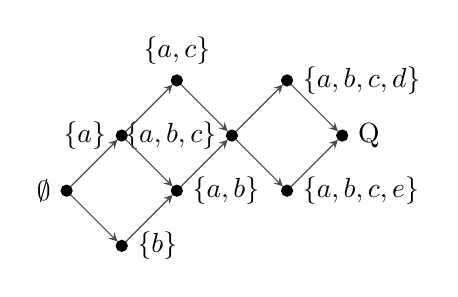
\begin{tikzpicture}
[
arc/.style={very thick},
state/.style={circle,draw=black,fill=black,inner sep = 0pt,
minimum size = 4pt},
scale=.7
]
\node[state,label=left:${\emptyset}$] (0) at (0,0){ };
\node[state,label=right:${\{b\}}$] (2) at (1,-1){ };
\node[state,label=left:${\{a\}}$] (1) at (1,1){ };
\node[state,label=right:${\{a,b\}}$] (12) at (2,0){ };

\node[state,label=above:${\{a,c\}}$] (13) at (2,2){ };
\node[state,label=left:${\{a,b,c\}}$] (123) at (3,1){ };
\node[state,label=right:${\{a,b,c,d\}}$] (1234) at (4,2){ };
\node[state,label=right:${\{a,b,c,e\}}$] (1235) at (4,0){ };
\node[state,label=right:Q] (12345) at (5,1){ };
\draw[-stealth,black!70] (0)--(1);
\draw[-stealth,black!70] (0)--(2);
\draw[-stealth,black!70] (1)--(12);
\draw[-stealth,black!70] (1)--(13);
\draw[-stealth,black!70] (2)--(12);
\draw[-stealth,black!70] (12)--(123);
\draw[-stealth,black!70] (13)--(123);
\draw[-stealth,black!70] (123)--(1234);
\draw[-stealth,black!70] (123)--(1235);
\draw[-stealth,black!70] (1234)--(12345);
\draw[-stealth,black!70] (1235)--(12345);
\end{tikzpicture}
\end{scriptsize}
\end{center}
\end{figure}
\end{frame}


\subsection{Algorithm}

\begin{frame}{
\includegraphics[scale=0.4]{Da_cambiare.png} \\ 
Flowchart of the Adaptive Assessment}{Doignon \& Falmagne, 1988; Donadello, et al., 2017} 
  \begin{columns}
     \column{0.5\textwidth}
   The goal of the assessment is to recover the {\color{blue}true state} of an individual asking the fewest possible questions
     \begin{itemize}
         \vspace{.2cm}
         \item Three rules guide the assessment:
         \vspace{.3cm}
         \begin{enumerate}
             \item Questioning rule
             \vspace{.2cm}
             \item Updating rule 
             \vspace{.2cm}
             \item Termination rule
         \end{enumerate}
         \vspace{.3cm}
        % \item The MSP1 assumption is used inside the updating rule
     \end{itemize}
     \column{0.5\textwidth}
     \begin{align*}
                   \vspace{-2cm}
    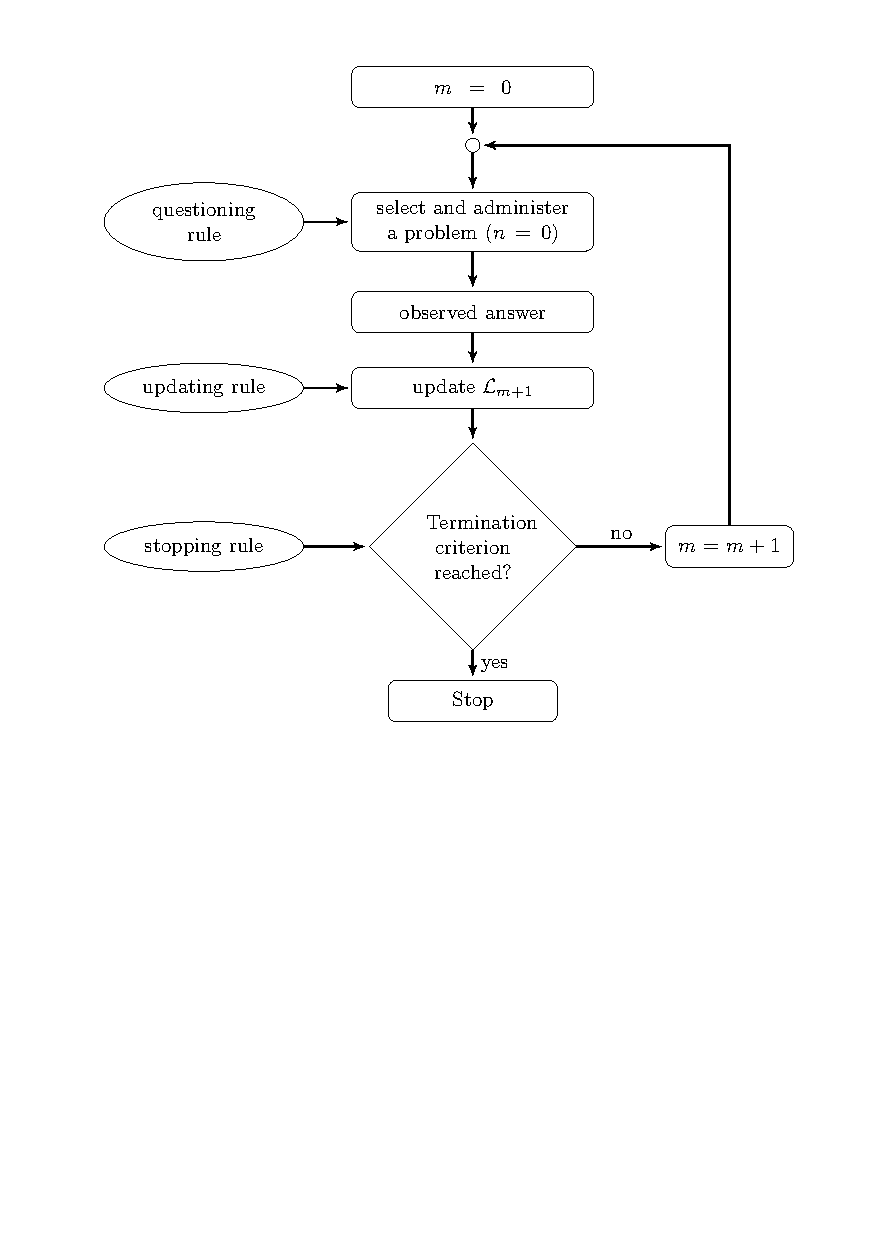
\includegraphics[scale=0.5]{Flowchart_cmp.pdf}
     \end{align*}
    \end{columns}
 
\end{frame}

\begin{frame}{
\includegraphics[scale=0.4]{Da_cambiare.png} \\ Probability distribution on the states}{} 
  \begin{columns}
     \column{0.5\textwidth}
 \footnotesize
A probability distribution 
\[\mathcal{L}_{m}: \mathcal{K} \rightarrow (0,1)\]

Without prior knowledge is a uniform distribution
\vspace{.5 cm}

  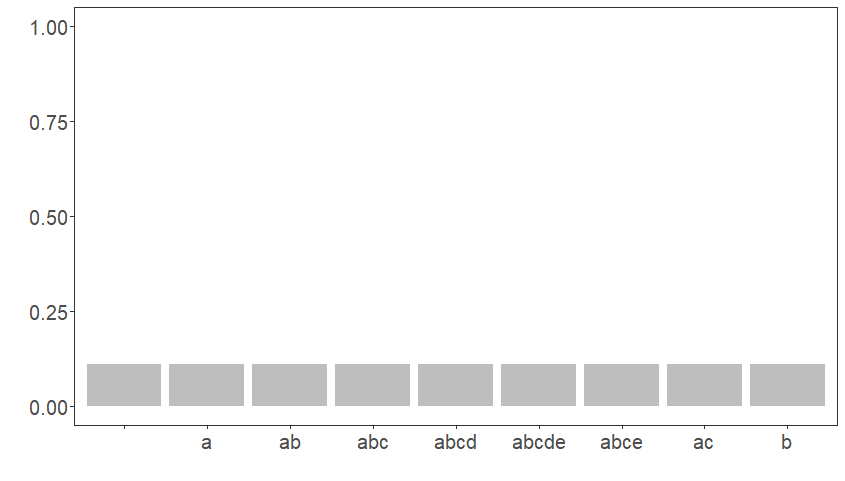
\includegraphics[scale=0.2]{Verosimiglianza.png}
   
     \column{0.5\textwidth}
     \begin{align*}
                   \vspace{-2cm}
    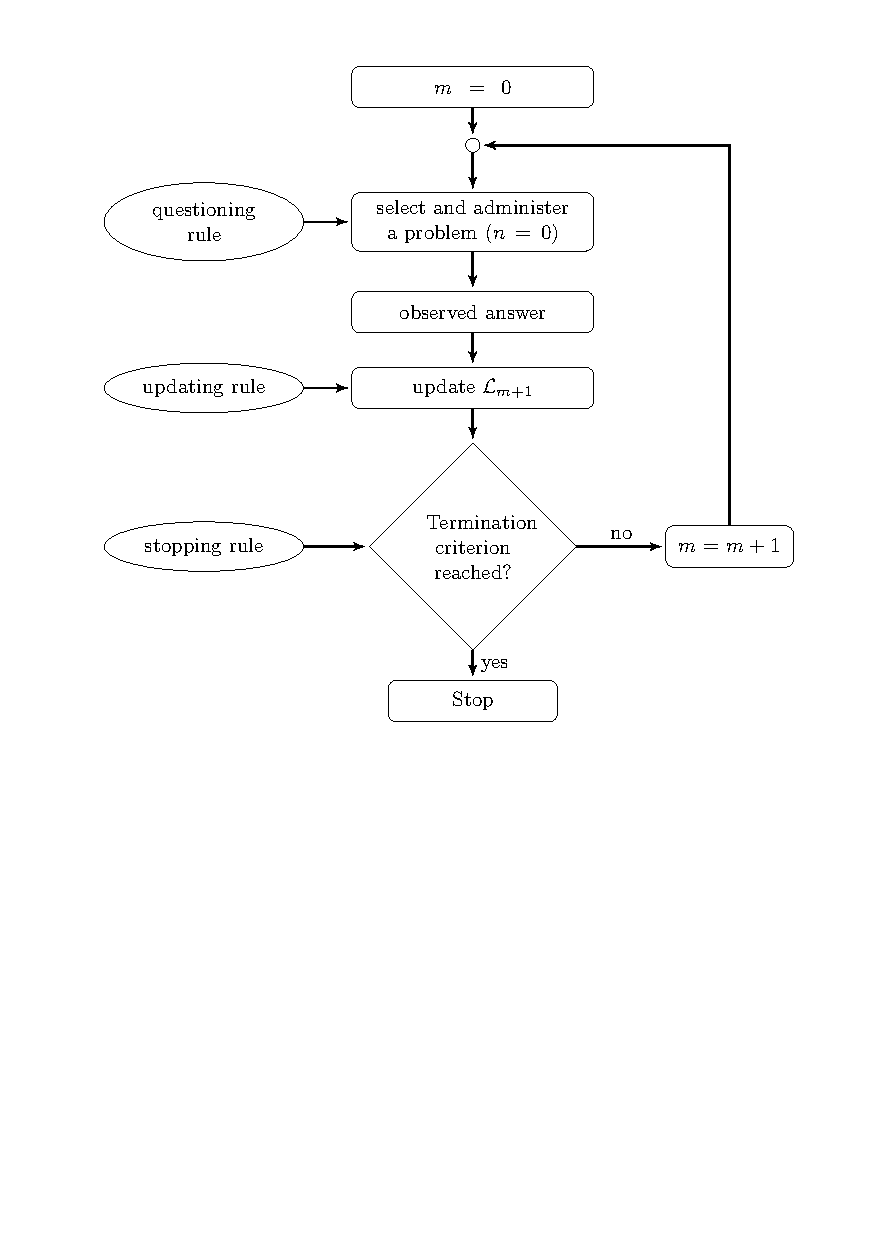
\includegraphics[scale=0.5]{Flowchart_cmp.pdf}
     \end{align*}
     \begin{tikzpicture}[overlay]
    \draw[red,ultra thick,rounded corners] (2.5,6.4) rectangle (4.5,6.7);
   \end{tikzpicture}
    \end{columns}
 
\end{frame}

\begin{frame}{
\includegraphics[scale=0.4]{Da_cambiare.png} \\ Questioning Rule }{ Half Split Rule} 
  \begin{columns}
     \column{0.5\textwidth}

Select the ``best'' question to ask \\
\vspace{.5cm}
\footnotesize
\begin{block}{Doignon \& Falmagne, 1988}
\texttt{half\_split:} Let $\mathcal{L}_m(K)$ the likelihood of $K$ at the step $m$, and the subset $\K_{q} \subset \K$ such that $q \in K$ for each $K \in K_{q}$. \\
It selected problem $q\in Q$ that minimize  
\[
|\mathcal{L}_m(\K_{q}) -1/2|
\]
\end{block}  
     \column{0.5\textwidth}
     \begin{align*}
                   \vspace{-2cm}
    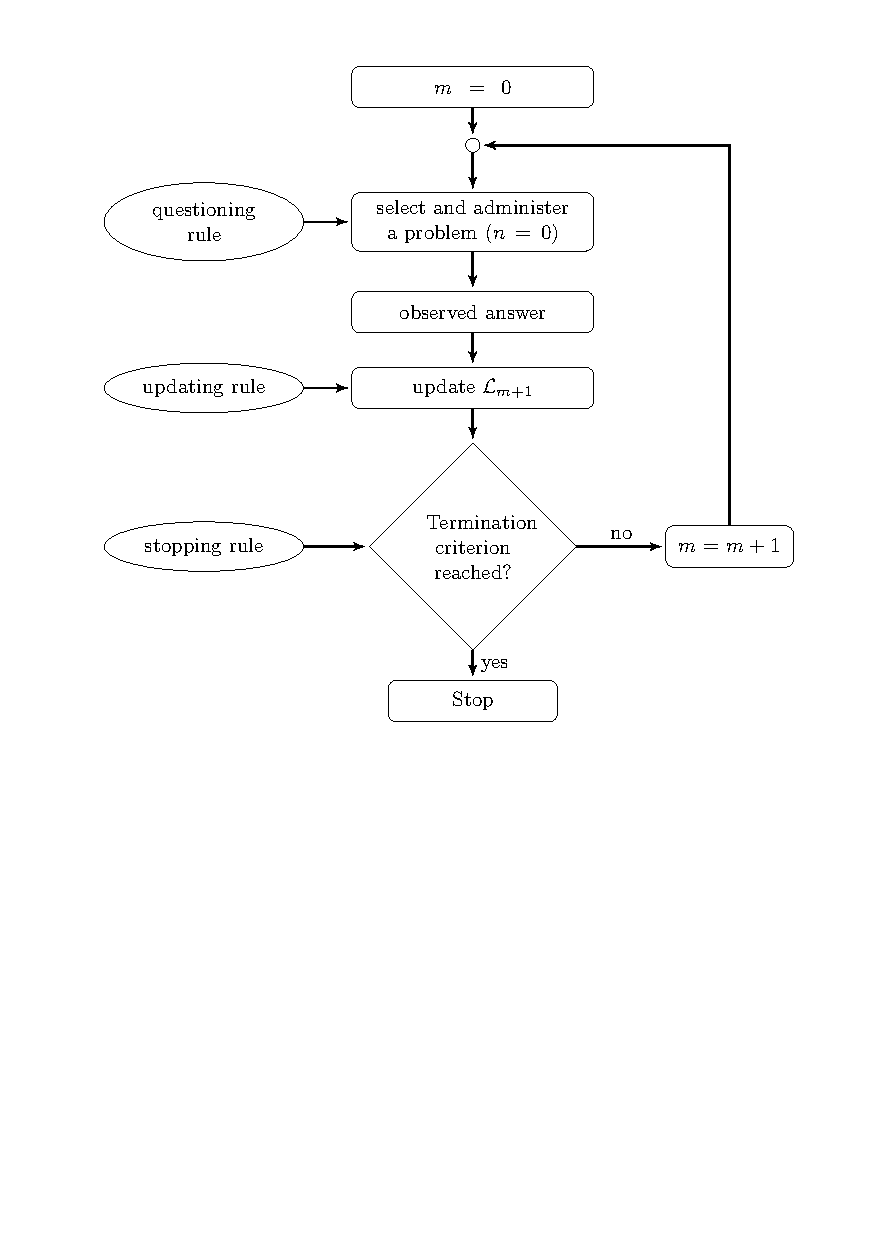
\includegraphics[scale=0.5]{Flowchart_cmp.pdf}
     \end{align*}
     
       \begin{tikzpicture}[overlay]
    \draw[red,ultra thick,rounded corners] (0.35,5) rectangle (2.1,5.8);
   \end{tikzpicture}
   
    \end{columns}
 
\end{frame}

\begin{frame}{
\includegraphics[scale=0.4]{Da_cambiare.png} \\ Updating Rule}{Bayesian Updating Rule} 
  \begin{columns}
     \column{0.5\textwidth}
\footnotesize
The probability $\mathcal{L}_{m}(K)$, for each $K \in \mathcal{K} $ is updated in function of the {\color{blue} the observed response} $r_q$ collected for problem $q$ as follows. 
\[
\mathcal{L}_{m+1}(K)=\frac{P(r_q|K) \mathcal{L}_{m}(K)}{\sum_{K' \in \K}P(r_q|K) \mathcal{L}_{m}(K')}
\]
\centering
\begin{scriptsize}

    \begin{block}{Parameters}
    \[
       P(r_q|K) = \begin{cases}
		\beta_{q} & \text{if  } r_q=0 \text{ \& } q \in K;\\
		1-\eta_{q} & \text{if  } r_q=0 \text{ \& } q \notin K;\\
		1-\beta_{q} & \text{if  } r_q=1 \text{ \& } q \in K;\\
		\eta_{q} & \text{if  } r_q=1 \text{ \& } q \notin K.\\
	\end{cases}
    \]
\end{block}
\end{scriptsize}

     \column{0.5\textwidth}
     \begin{align*}
                   \vspace{-2cm}
    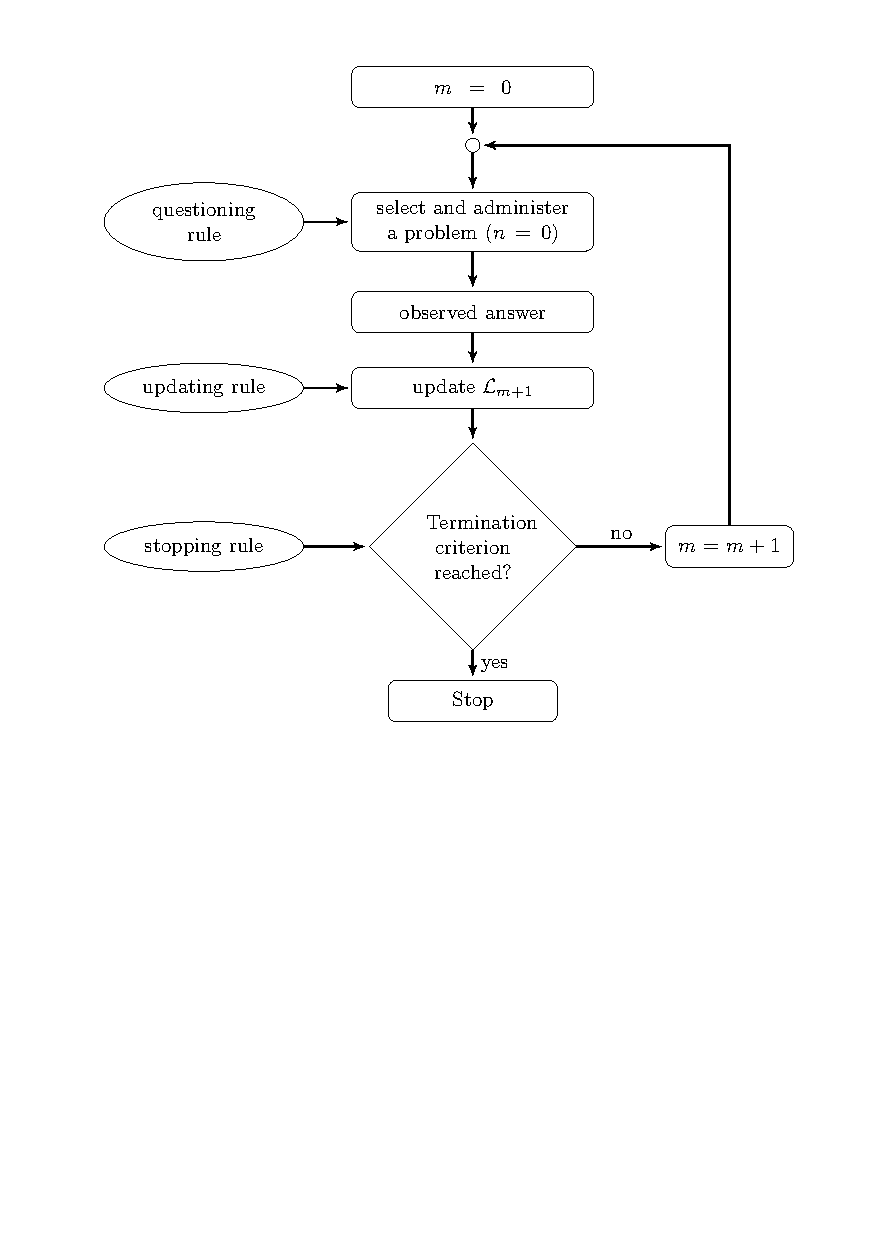
\includegraphics[scale=0.5]{Flowchart_cmp.pdf}
     \end{align*}
            \begin{tikzpicture}[overlay]
    \draw[red,ultra thick,rounded corners] (0.35,3.7) rectangle (2.1,4.3);
   \end{tikzpicture}
   
    \end{columns}
 
\end{frame}


\begin{frame}{
\includegraphics[scale=0.4]{Da_cambiare.png} \\ Termination rule}{ } 
  \begin{columns}
     \column{0.5\textwidth}
\footnotesize
\begin{block}{Heller \& Repitsch, 2012 }
 \texttt{Likelihood Maximization: }The assessment terminate at step $m$ if 
\[
\max\mathcal{L}_{m}(K) > SC
\]
with $SC \in (0.5,1]$. 
\end{block}

\begin{block}{Donadello, et al., 2017 }
\texttt{Item Discrimination: }The assessment terminate at step $m$ if for each $q \in Q$
\[
\mathcal{L}_{m}(\mathcal{K}_q) > SC \text{ or } \mathcal{L}_{m}(\mathcal{K}_q) < 1-SC
\]
with $SC \in [0.5,1]$. 
\end{block}


     \column{0.5\textwidth}
     \begin{align*}
                   \vspace{-2cm}
    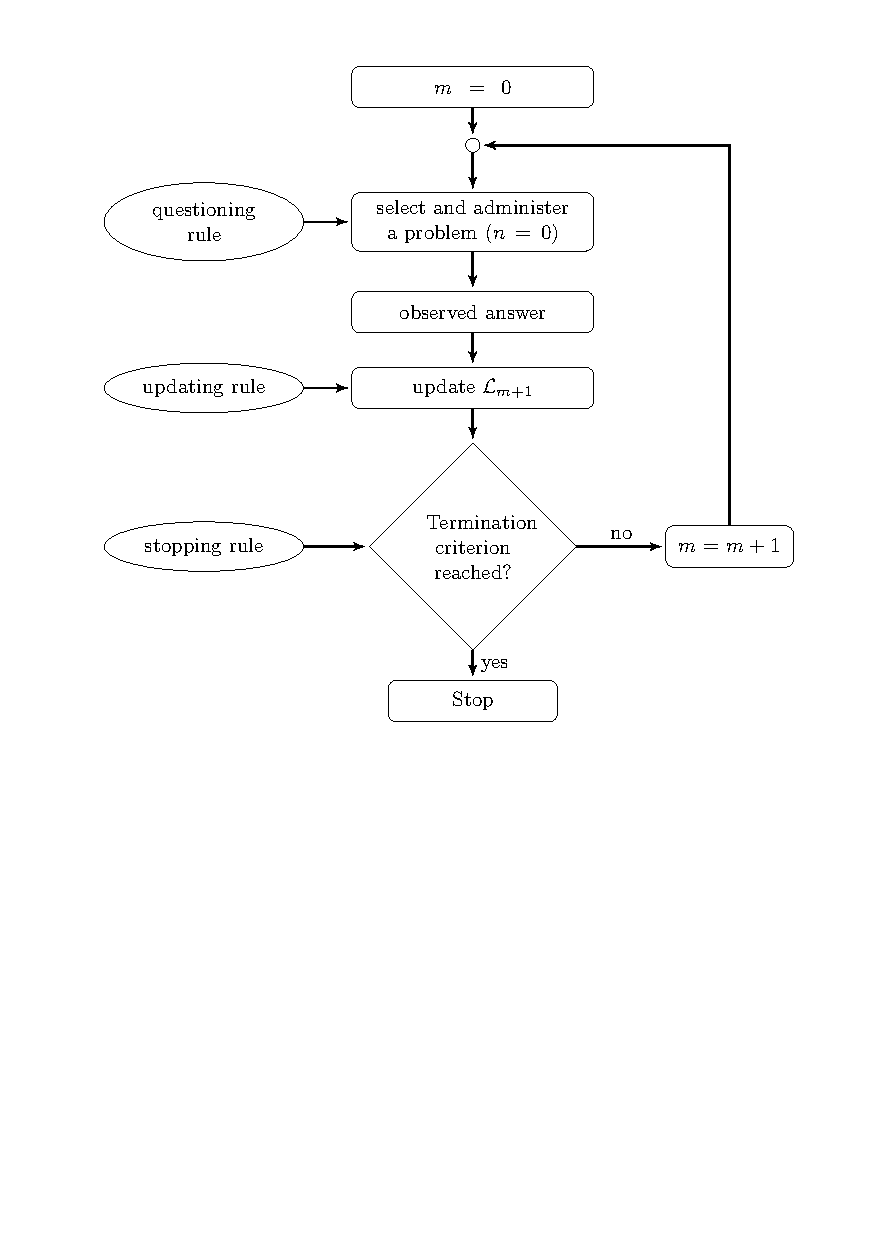
\includegraphics[scale=0.5]{Flowchart_cmp.pdf}
     \end{align*}
                 \begin{tikzpicture}[overlay]
    \draw[red,ultra thick,rounded corners] (0.35,2.38) rectangle (2.1,2.9);
   \end{tikzpicture}
   
    \end{columns}
 
\end{frame}

\subsection{Shiny}
\begin{frame}{
\includegraphics[scale=0.4]{Da_cambiare.png} \\ 
Create and Try the Test ... }{... without coding 
 knowledge \texttt{run\_Practice()}}
\only<1>{
  \vspace{.5cm}

\includegraphics[scale=0.17]{Intro.png}}
 \only<2>{ 
   \vspace{.5cm}
 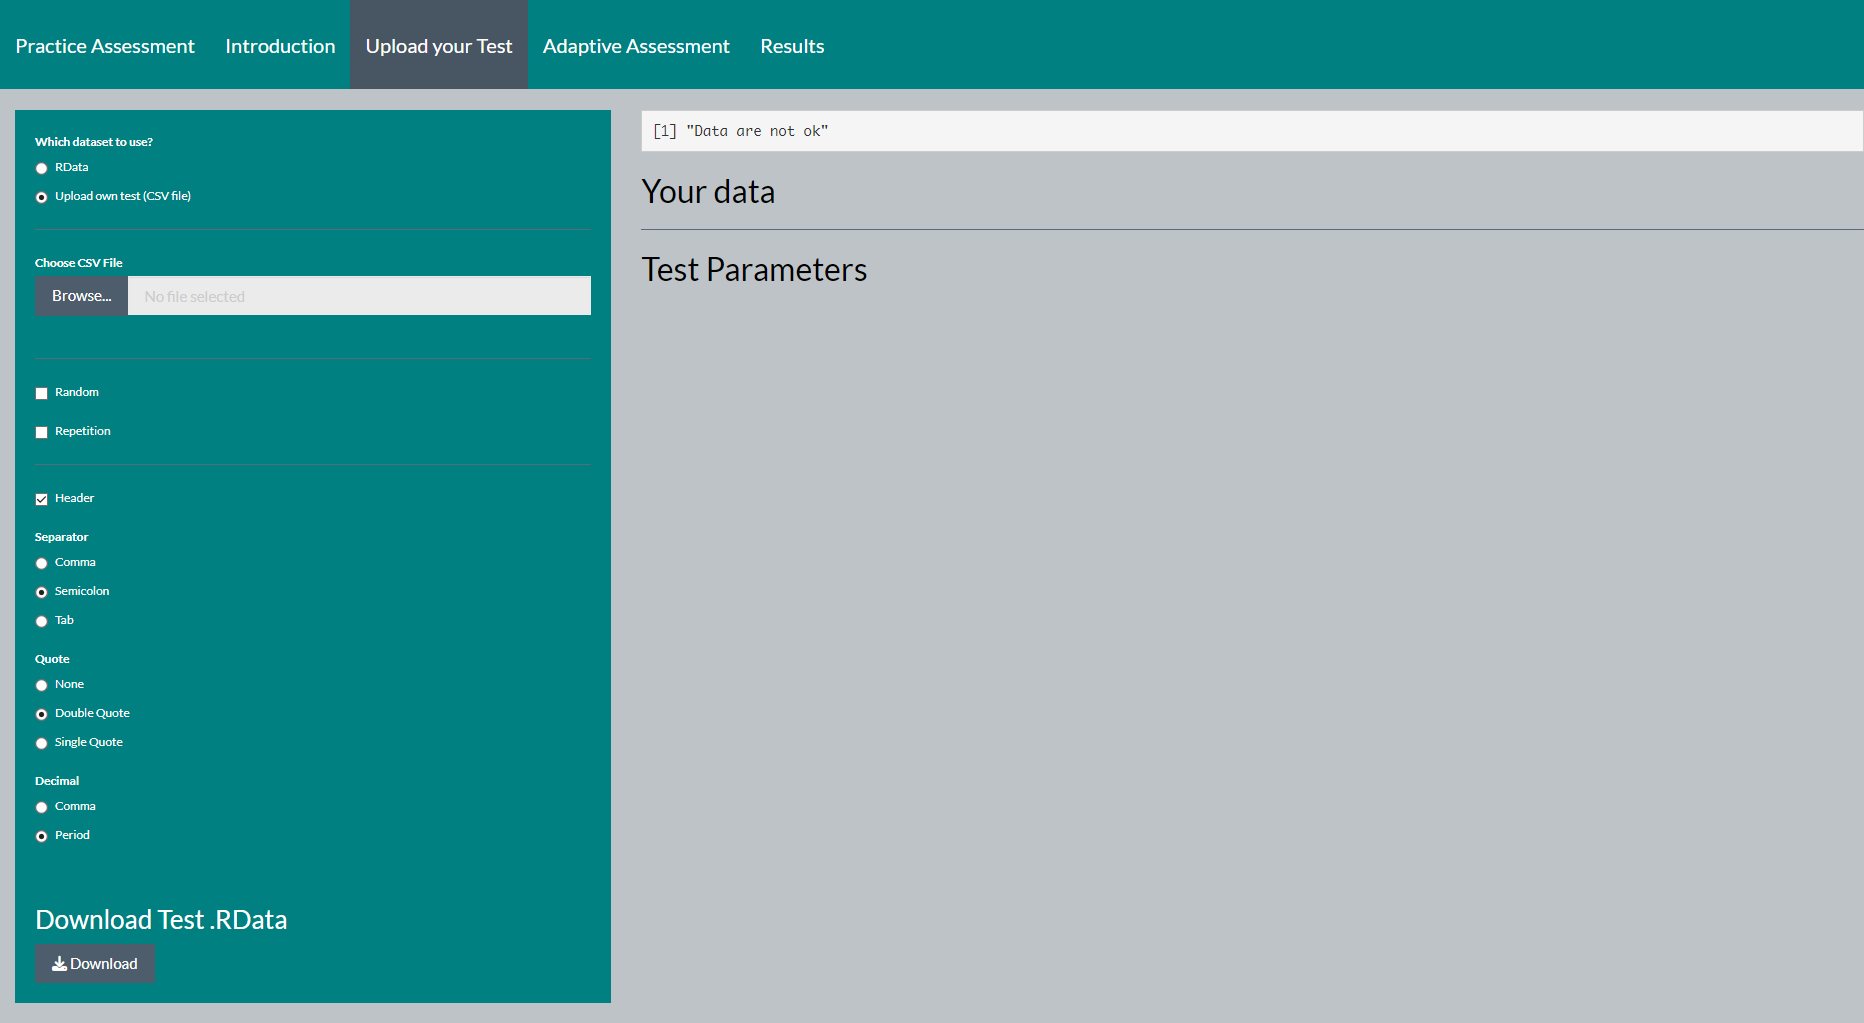
\includegraphics[scale=0.16]{Loadtest.png}}
   \only<3>{
   \vspace{.5cm}
 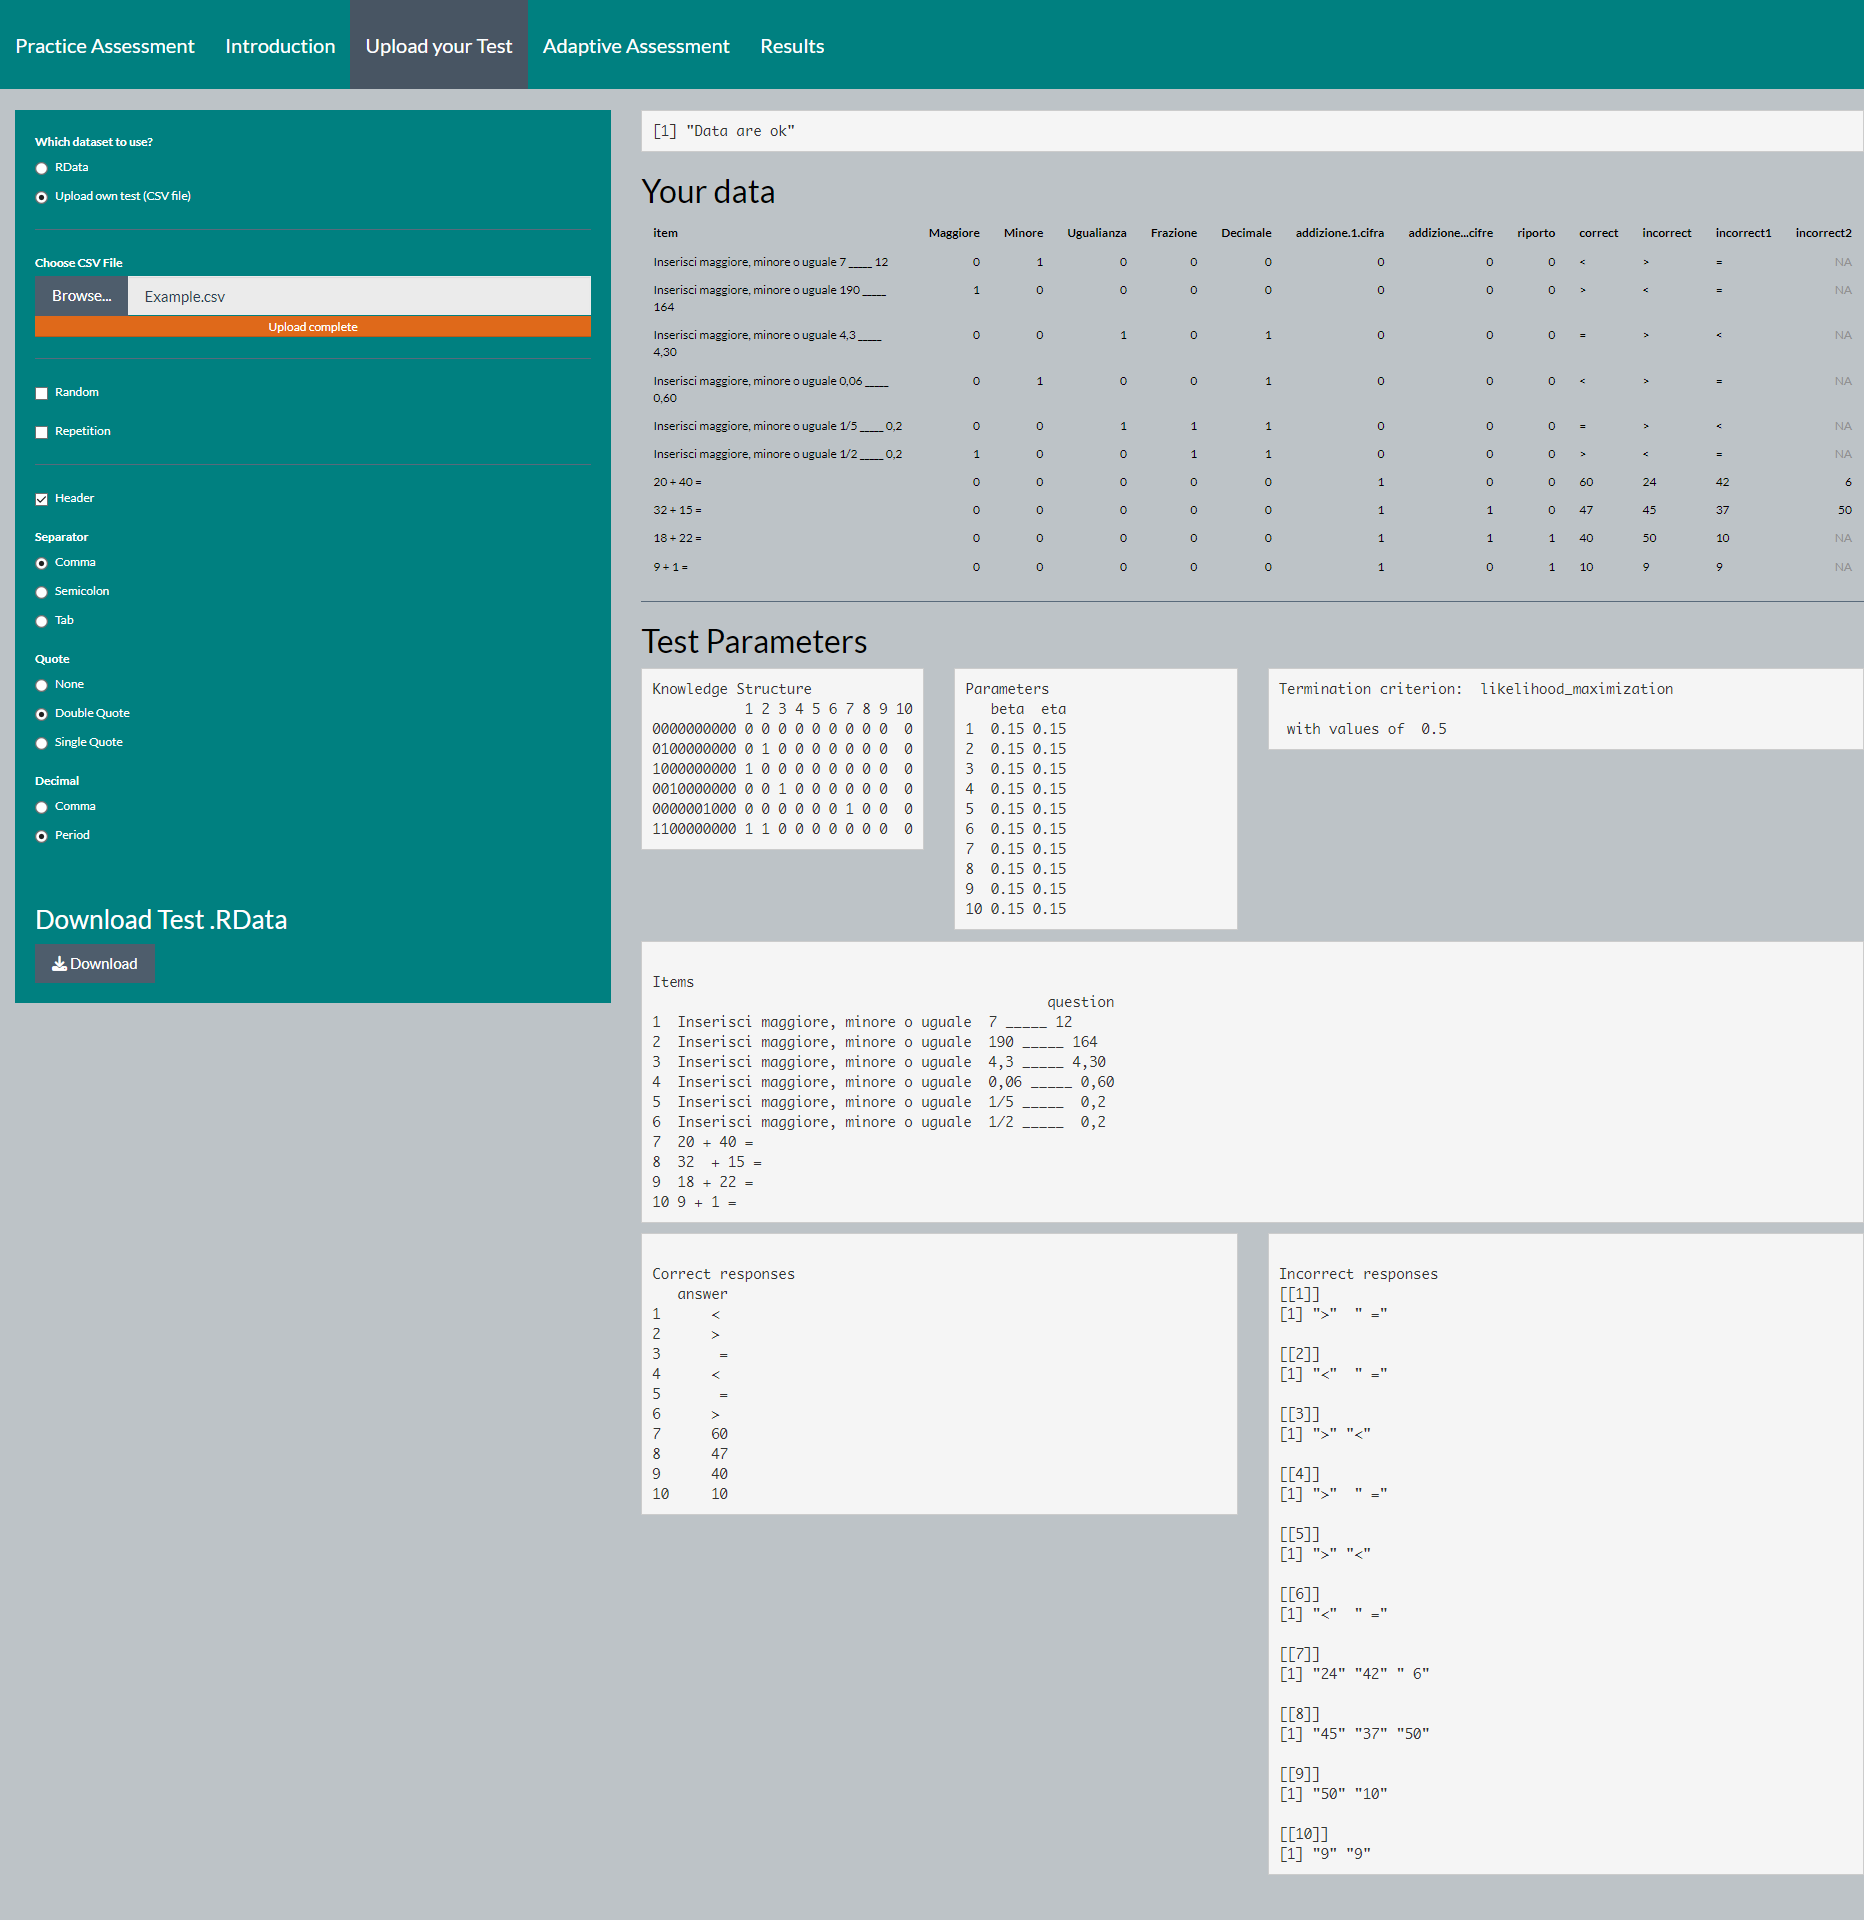
\includegraphics[scale=0.16]{Loadtest2.png}}
 \only<4>{ 
   \vspace{.5cm}
 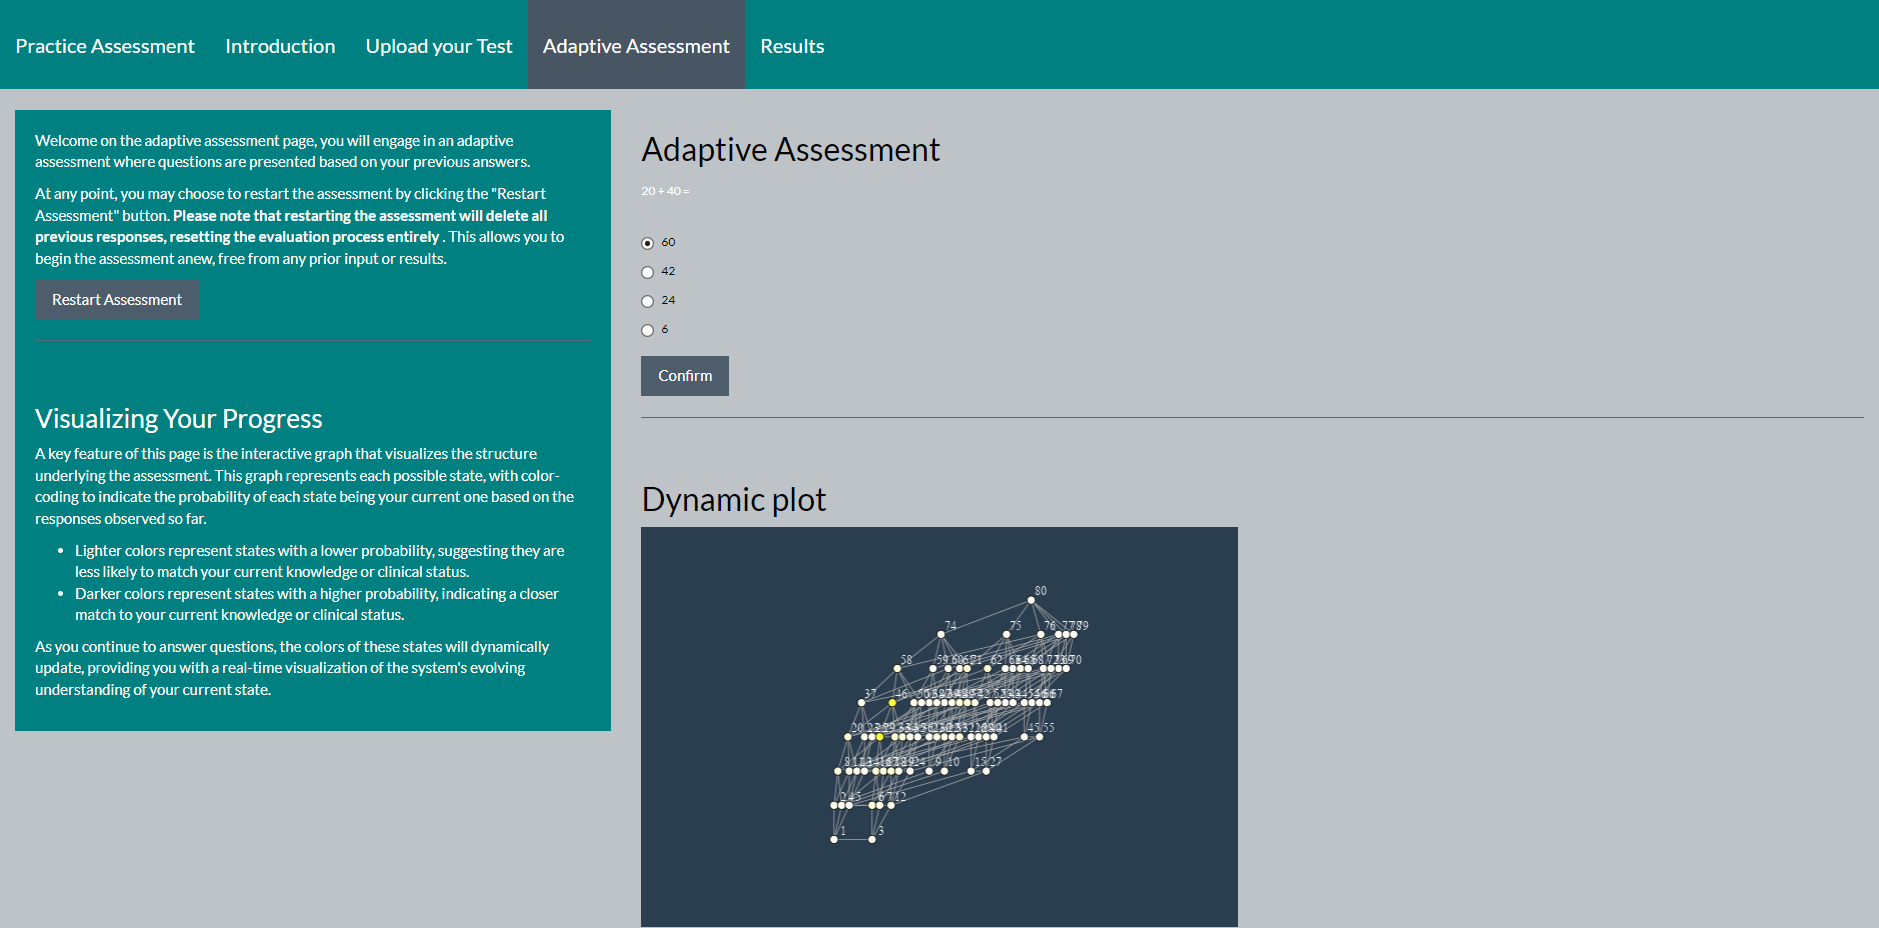
\includegraphics[scale=0.15]{Assessment.png}}
  \only<5>{ 
    \vspace{.5cm}
 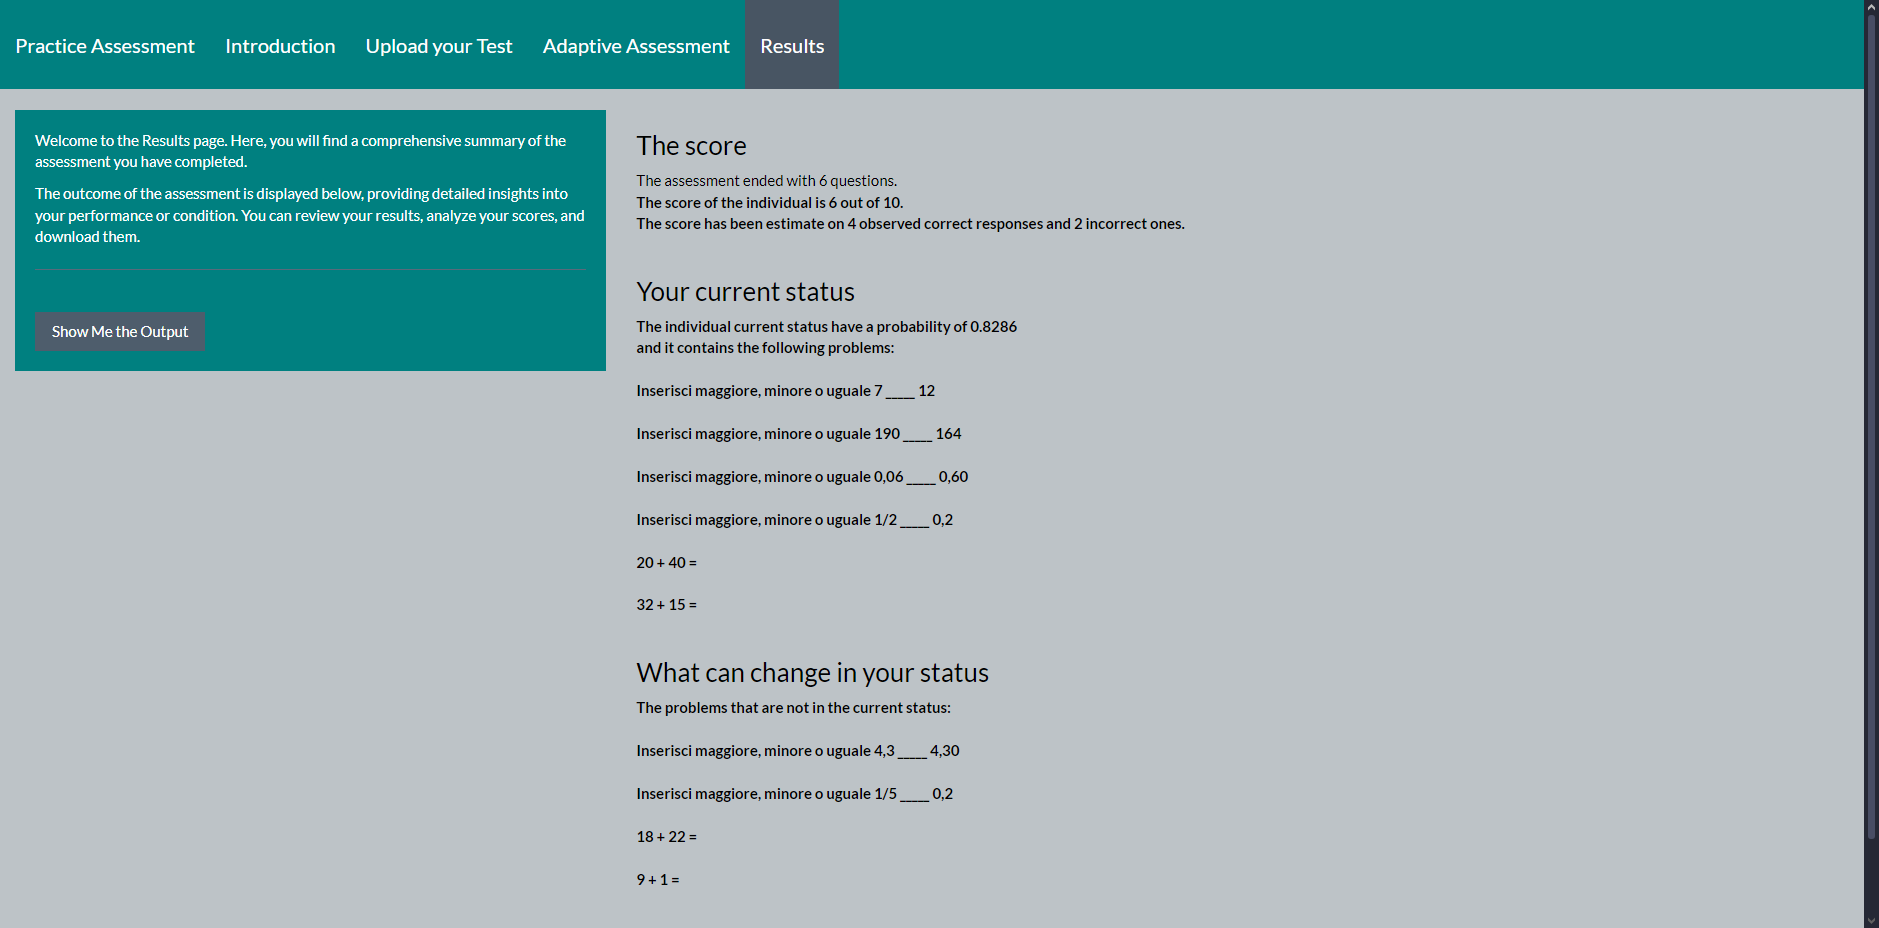
\includegraphics[scale=0.15]{outcome.png}}
\end{frame}


\subsection{Application on RAISE}
\begin{frame}{
\includegraphics[scale=0.4]{Da_cambiare.png} \\ RAISE - Robotics and AI for Socioeconomic Empowerment}{}
\begin{itemize}
    \item In collaboration with some middle schools in Lombardia and Liguria
    \vspace{.1cm}
    \item A pilot test covering the middle school program in in mathematics
    \vspace{.1cm}
    \end{itemize}
    \onslide<2->{
   \begin{block}{Tuning a Test with mycaas}
    21 items with multiple choice and 595 states
    \vspace{.1cm}\\
    Simulation parameters: 
     \begin{itemize}
         \item two termination rules with six stopping criteria $SC= \{.5,.6,.7,.8,.9,1\}$ 
         \item simulate ten response patterns for each $K \in \mathcal{K}$
         \item lucky guess $\eta_q = .2$ \& careless error $\beta_q =.15$ 
     \end{itemize}
     
\end{block}
  }
\end{frame}

\begin{frame}{
\includegraphics[scale=0.4]{Da_cambiare.png} \\ 
Performance Analysis}{Accuracy and Efficiency Indexes}
\footnotesize
    \begin{block}{Given:}
    \begin{itemize}
        \item true knowledge state $K^w$ of a student $w$;
        \item the probability distribution $\mathcal{L}_{m}$ at the end of the assessment
        \item the recovered knowledge state $\hat{K}_m^w$ 
    \end{itemize}
    \end{block}
    \vspace{.2cm}
The following indexes were computed across simulated subjects: 
    \vspace{.2cm}
\begin{enumerate}
\item The {\color{blue}average number of questions asked}.
\item The {\color{blue}average maximum likelihood} $\bar{\mathcal{L}}_m ( \hat{K}_m )$.
	\item The {\color{blue}average Hamming distance} $\bar{D}_m(K,\hat{K}_m)$
	computed by
\[
\bar{D}_m(K,\hat{K}_m)=\frac{1}{N}\sum_{w=1}^N |K^w \Delta \hat{K}_m^w|,
\]
where $\Delta$ represents the symmetric set difference.

\end{enumerate}
\end{frame}

\begin{frame}{
\includegraphics[scale=0.4]{Da_cambiare.png} \\ 
Performance Analysis}{\texttt{performance\_simulation(\dots)}}
    \begin{columns}
     \column{0.50\textwidth}
     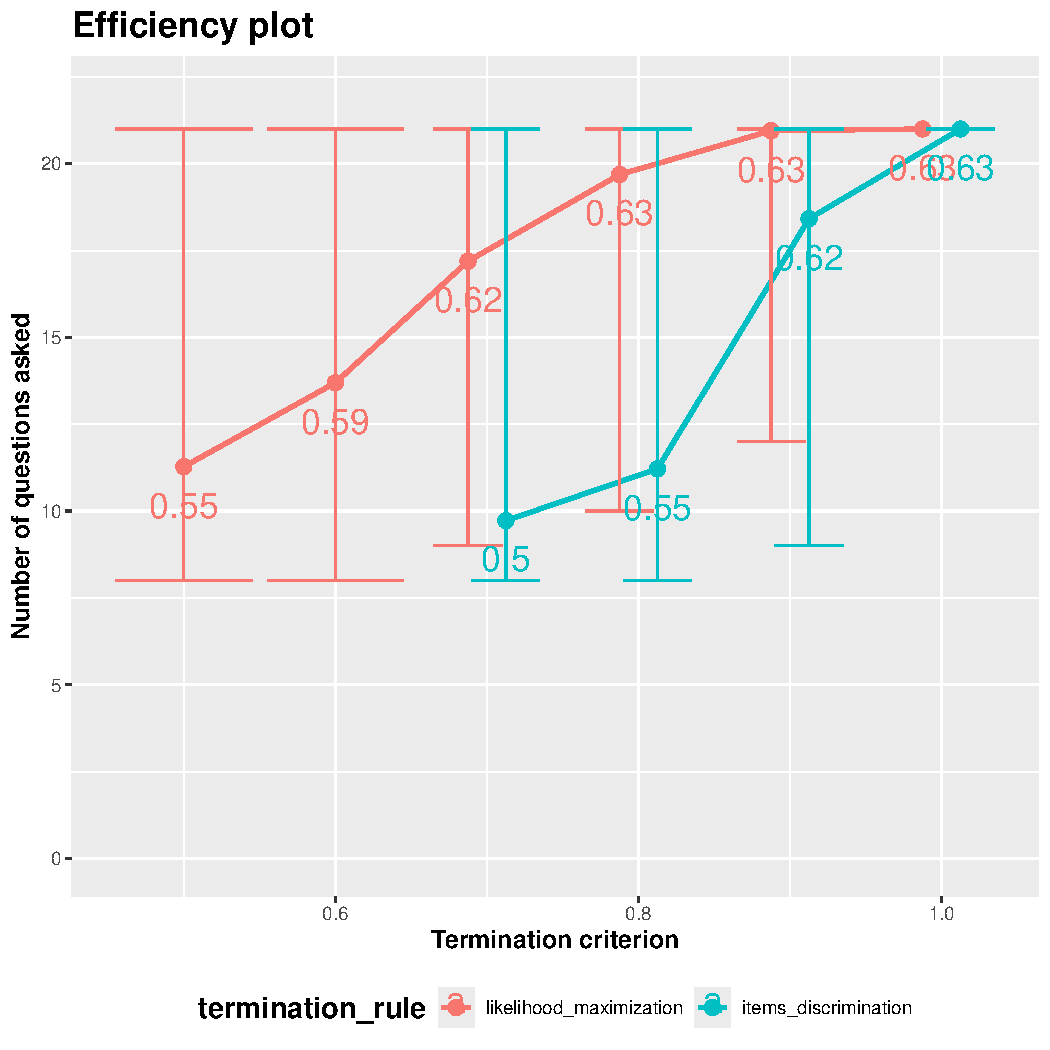
\includegraphics[scale=0.3]{Efficiency.pdf}
     \column{0.50\textwidth}
      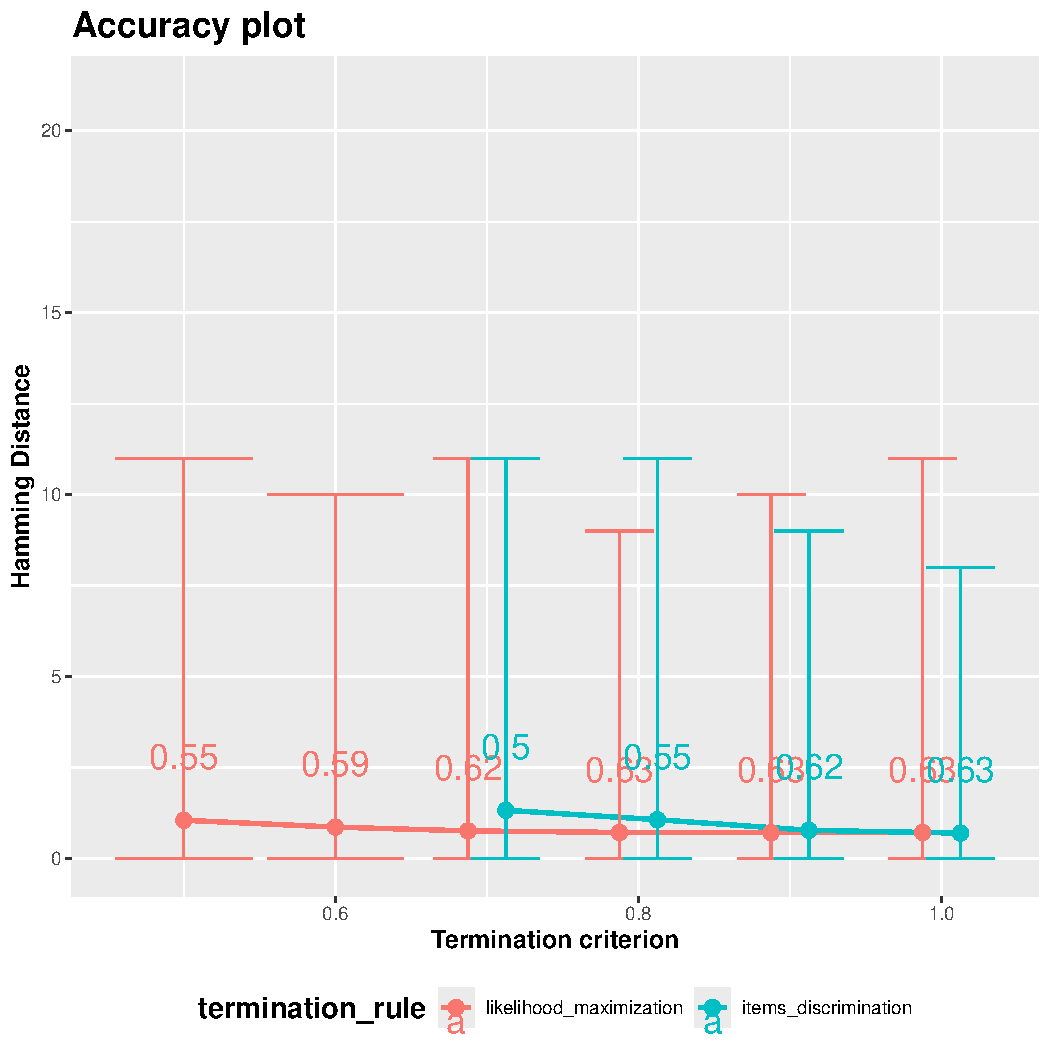
\includegraphics[scale=0.3]{accuracy.pdf}   
     \end{columns}
\end{frame}


\section{Final Remarks}

\begin{frame}{
\includegraphics[scale=0.4]{Da_cambiare.png} \\ 
Cons of Adaptive Assessment}
\small
\begin{itemize}
    \item Dependent on the assumptions of the Model :
    \begin{itemize}
        \item The validity of results depends on the correctness of the model used.\\ 
         \only<2->{\item \textcolor{blue}{Response}: Building upon KST and FPA}
    
    \end{itemize}
     \vspace{.3 cm}
    \item  Complexity of Implementation:
    \begin{itemize}
        \item Requires sophisticated algorithms and data processing infrastructure.
    
         \only<4->{\item \textcolor{blue}{Response}: GUI offline interface for adaptive assessment  \texttt{run\_Assessment()} and \texttt{run\_Practice()}}
    \end{itemize}
     \vspace{.3 cm}
    \item Difficulty in Tuning:
    \begin{itemize}
        \item Fine-tuning the assessment to achieve accurate difficulty adjustments is challenging.
        \only<6->{\item \textcolor{blue}{Response}: Performance analysis of the test \texttt{performance\_simulation()}}
    \end{itemize}
\end{itemize}
\end{frame}

\begin{frame}{
\includegraphics[scale=0.4]{Da_cambiare.png} \\ 
Final Remarks}{}
 \begin{itemize}
 \item   The Shiny environment is used to make adaptive assessments more accessible and user-friendly.\\
   \vspace{.1cm}
 \item  Currently the usability of the package is tested within RAISE in Liguria school\\
  \vspace{.1cm}
 \item \texttt{https://github.com/brancaccioandrea/mycass}
  \end{itemize}
  \begin{center}
  
\includegraphics[scale=0.25]{qr.pdf}
  \end{center}
  
   \end{frame}
   
\begin{frame}{
\includegraphics[scale=0.4]{Da_cambiare.png} \\ 
Acknowledgements:}{}
 
 
This work has been supported by the European Commission, NextGenerationEU, Missione 4 Componente 2, “Dalla ricerca all’impresa”, Innovation Ecosystem RAISE “Robotics and AI for Socio-economic Empowerment”, ECS00000035.


\end{frame}
\end{document}